\section{Marching Cubes} \label{sec:theory_theory_marching_cubes}
One of the requirements for our project was to incorporate terrain generation.
Numerous algorithms exist for this purpose, and the chosen algorithm for our project is known as marching cubes.
This algorithm was selected due to its simplicity, versatility, and standardization.
Marching cubes is a relatively straightforward algorithm that can be easily modified to suit different requirements, as explained in detail in \autoref{sec:system_architecture_terrain_generation}.
Furthermore, it is widely used in various applications and is well-documented, making its understanding and implementation easier.

The concept of marching cubes was first introduced by William E. Lorensen and Harvey E. Cline in 1987 \cite{Marching-Cubes}.
The fundamental idea behind this algorithm is to generate a mesh from a scalar field.
An isolevel is chosen, 0 being the most common choice and the one we used.
Points with values greater than the isolevel are considered to be "above" the surface, while points with values lower than the isolevel are considered to be "below" the surface.
The world is divided into cubes, and for each cube, the algorithm determines which of its vertices are above and below the surface.
Based on this information, a mesh is created to separate the vertices above the surface from those below it.
An example of this process is illustrated in \autoref{fig:cube_example}, where $v0$ is below the surface, while the remaining vertices are above it.
It is important to note that the same effect would be achieved if $v0$ were above the surface and the other vertices were below it.

\todo{Can we use images found online? If so how do we cite them?}
\begin{figure}[H]
    \centering
    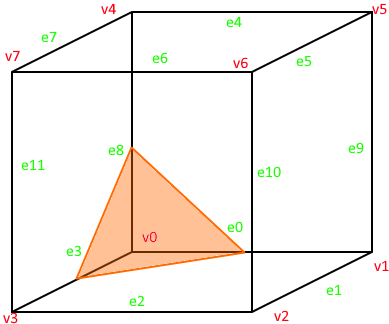
\includegraphics[width=0.5\textwidth]{chapters/theoretical_foundations/sections/marching_cubes/resources/cube-example.png}
    \caption["Marching" cubes with only $v0$ below the surface.]{"Marching" cubes with only $v0$ below the surface. Source: \url{https://polycoding.net/marching-cubes/}}
    \label{fig:cube_example}
\end{figure}

Each cube consists of 8 vertices, and each vertex is classified as either above or below the surface, resulting in a total of 256 possible combinations.
However, there are only 15 unique combinations, all of them depicted in \autoref{fig:marching_cubes_configurations}, with the remaining combinations being rotations and reflections of these 15 cases.
For each of these unique combinations, a precomputed table is utilized to generate the corresponding mesh.
This table provides information about which edges of the cube are intersected by the surface and how to connect them.

\begin{figure}[H]
    \centering
    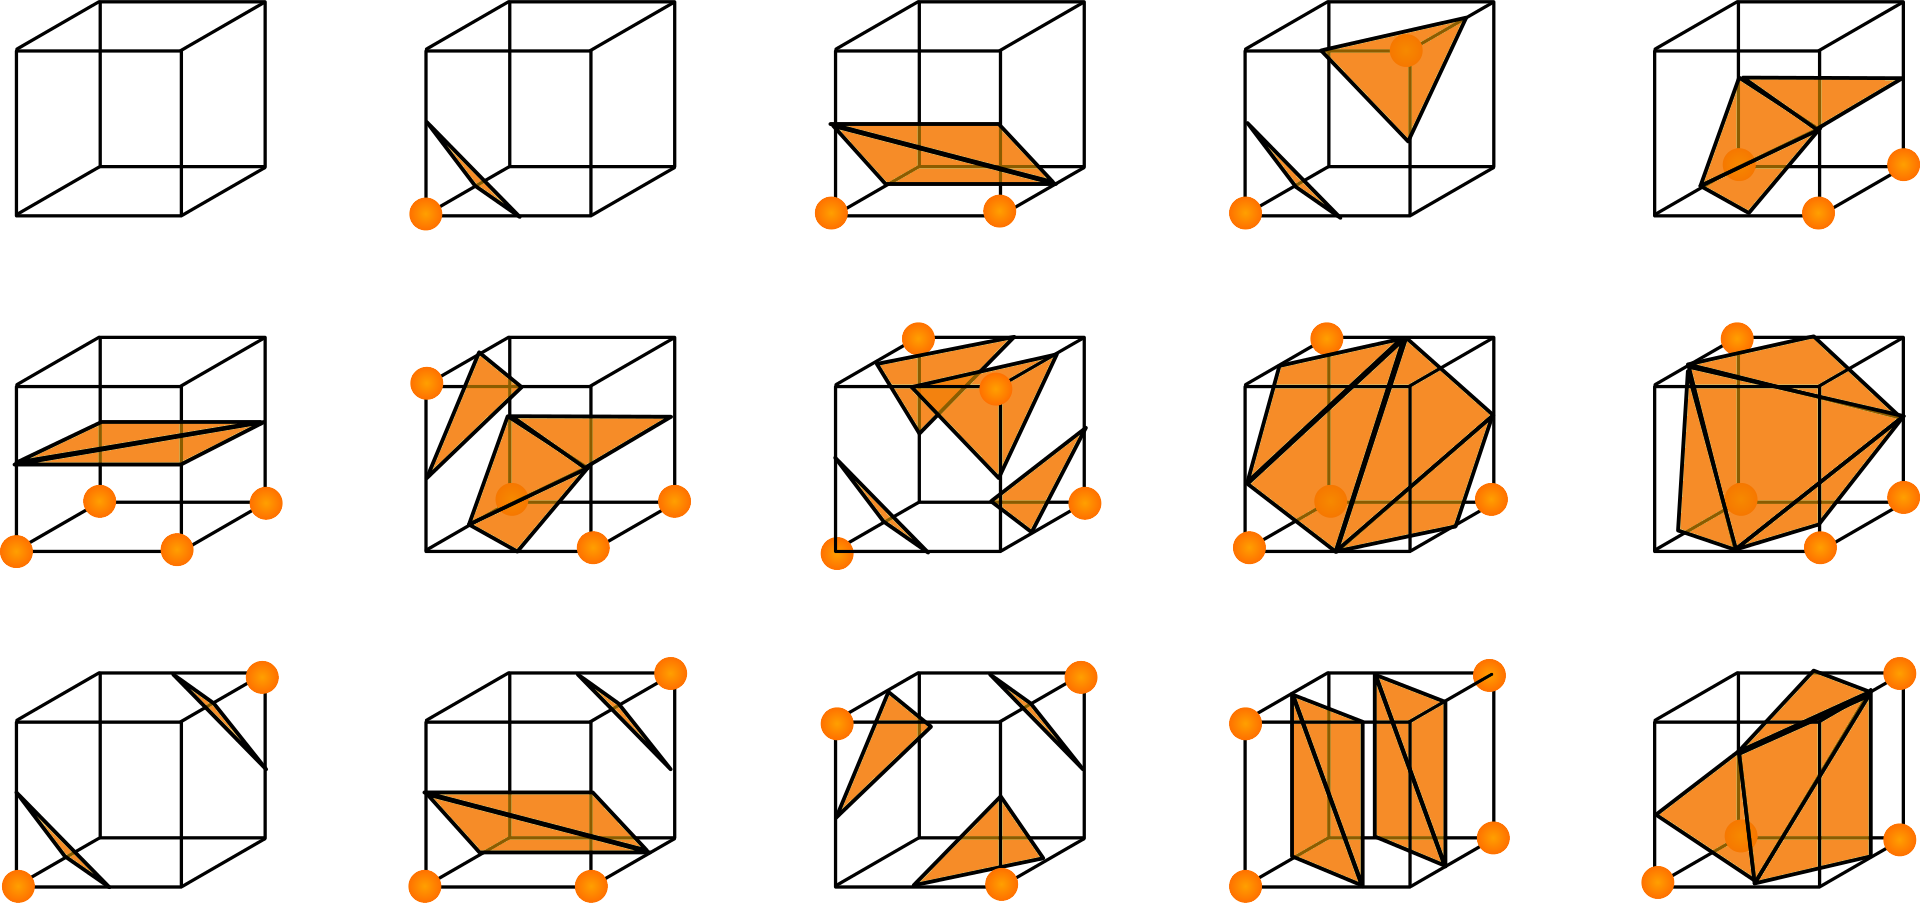
\includegraphics[width=0.8\textwidth]{chapters/theoretical_foundations/sections/marching_cubes/resources/marching-cubes-configurations.png}
    \caption[Unique marching cubes configurations]{Unique marching cubes configurations. Source: \url{https://polycoding.net/marching-cubes/}}
    \label{fig:marching_cubes_configurations}
\end{figure}
